% Generated from arXiv:2512.24528; see tools/build_source_compendium.py.
\section{Calculation laboratory VII: Encircling an exceptional resonance}
\label{lab:2512_24528}

\calculationroute
  {Complex-scaled left and right eigenvectors, a second-order exceptional point, Jordan chains, and Berry holonomy.}
  {The complex-scaled Rosen--Morse eigenfunctions, self-orthogonality, branch exchange, geometric phase, Chern data, monodromy renormalization, and momentum-bin continuum states.}
  {Track the branch exchange, self-orthogonality, and geometric phase through an EP while separating bin normalization from the holonomy.}

This Laboratory reconstructs the calculation underlying
Ref.~\cite{Morikawa:2025inx}.  Resonance boundary conditions and the ABC
theorem are referenced from Stages II and IV.  We retain the solvable
Rosen--Morse eigenfunction because it is the input from which the EP
derivatives and holonomy are calculated.

\begin{comment}
\subsection{Resonance wave function in complex-scaling method}
\subsubsection{Complex scaling and the ABC theorem}
Resonances in scattering correspond to poles of the S matrix at complex energies
\begin{equation}
 E = \resonantE - \frac{\rmi}{2}\Gamma,
\end{equation}
where $E_{R}$ is a resonant energy, and $\Gamma>0$ is a decay width.
A resonance wave function is characterized by the purely outgoing (Siegert) boundary condition~\cite{Siegert:1939}. 
In one-dimensional scattering, the outgoing solutions behave asymptotically as
\begin{equation}
\psi(x)\sim
\begin{cases}
\rme^{+\rmi kx} & x\to +\infty,\\
\rme^{-\rmi kx} & x\to -\infty,
\end{cases}
\end{equation}
with a complex wave number $k=\sqrt{2mE}/\hbar$.
Because $\mathrm{Im}\,k\neq 0$ in general, such solutions diverge exponentially in at least one direction and are not square integrable,
\begin{equation}
\psi \notin L^2(\mathbb{R}).
\end{equation}
Standard methods determine reflection and transmission for real $E$, but do not by themselves turn resonance poles into a discrete, well-posed eigenvalue problem.
The complex-scaling method (CSM) provides a framework that exposes resonance poles as discrete eigenvalues. 
One performs the complex coordinate rotation
\begin{equation}
x \mapsto x \rme^{\rmi \theta},\qquad 0<\theta<\frac{\pi}{4},
\end{equation}
implemented by a nonunitary transformation $U_\theta$,
which maps the Hamiltonian $H$ to the complex-scaled operator
\begin{equation}
H_\theta = U_\theta H U_\theta^{-1}.
\end{equation}
Operationally, complex scaling has two key consequences: (i) purely outgoing resonance solutions, which are non-$L^2$ on the real axis, become square integrable after scaling, and (ii) resonances can be computed as discrete eigenpairs $(E,\psi_\theta)$ of $H_\theta$, rather than being inferred indirectly from peaks or rapid phase variations on the real energy axis.
The mathematical basis for these statements is provided by the Aguilar--Balslev--Combes (ABC) theorem~\cite{Aguilar:1971ve,Balslev:1971vb}, 
which implies the following properties of $H_\theta$:
\begin{enumerate}
    \item \textit{Square integrability of resonances.} Resonant solutions are represented by $L^2$ eigenfunctions of $H_\theta$, similarly to bound states.
    \item \textit{$\theta$ stability.} Bound-state energies and resonance eigenvalues are invariant under variations of the scaling angle $\theta$ within an analyticity sector.
    \item \textit{Rotation of the continuum.} The continuous spectrum, starting from physical threshold energies, is rotated clockwise by an angle $2\theta$ from the positive real axis in the complex energy plane.
\end{enumerate}
Thus, at finite $\theta$ the resonance problem is reduced to a discrete (non-Hermitian) eigenvalue problem for $H_\theta$.
\end{comment}
\subsection{The solvable resonance family used at the exceptional point}
\subsubsection{Solving method within complex-scaling method}
Our considerations in this paper will be applicable quite generically to scattering theory in one dimension. To illustrate it, we show explicit computations in an exactly solvable model: the inverted Rosen--Morse potential or P\"oschl--Teller potential. It is well known that this system supports barrier resonance.
For the inverted Rosen--Morse potential, the Schr\"{o}dinger equation under the CSM is given by
\begin{align}
    \left[-\frac{\hbar^2}{2m} \frac{\rmd^2}{\rmd x'^2} + \frac{\lambda}{\cosh^2 \beta x'}\right] \psi(x')
    = E \psi(x') ,
    \label{src:2512_24528:eq:CSM-eq}
\end{align}
where we have replaced $x\in\mathbb{R}$ by $x'=xe^{\rmi \theta}\in\mathbb{C}$ with the scaling angle $\theta$ and assume $\lambda>0$.
$m$ is the mass parameter, $\lambda$ and $\beta$ determine the height and the width of the potential, respectively.
For simplicity---namely, to identify the differential equation with a hypergeometric-type equation---we introduce several somewhat technical but convenient variables.
%The range of $\theta$ is restricted to $0<\theta<\pi/4$ in the CSM. 
Letting $\xi=\tanh\beta x'$, the equation is represented as
\begin{align}
    \left[ \frac{\rmd}{\rmd \xi} (1-\xi^2)\frac{\rmd}{\rmd \xi} +s(s+1) - \frac{\kappa^2}{1-\xi^2} \right] \psi(x')
    = 0 ,\\
    \kappa = \frac{\sqrt{-2mE}}{\beta\hbar},
    \qquad
    s = \frac{1}{2} \left(-1 + \sqrt{1-\frac{8m\lambda}{\beta^2\hbar^2}}\right).
    \label{src:2512_24528:eq:CSM-reduced-eq}
\end{align}
Substituting $\psi(x')=(1-\xi^2)^{\frac{\kappa}{2}}\omega(\xi)$ into Eq.~\eqref{src:2512_24528:eq:CSM-reduced-eq}, we obtain the hypergeometric differential equation explicitly in terms of~$\beta$, $\kappa$, $s$, and $u$
\begin{align}
    u(1-u)\omega''+(\kappa+1)(1-2u)\omega'
    -(\kappa-s)(\kappa+s+1)\omega&=0,
    \\
    u&=\frac{1-\xi}{2}.
\end{align}
Here primes denote derivatives with respect to~$u$.
The solution of this equation, which is regular at $x=0$, is given by
\begin{align}
    \vsub{\psi}{CSM}(x)= (1-\xi^2)^{\frac{\kappa}{2}} 
    F\left( \kappa-s, \kappa+s+1, \kappa+1, \frac{1-\xi}{2} \right).
\end{align}
Here, $F$ is the Gauss hypergeometric function.
In general, as $x\to-\infty$ ($\xi\to-1$), the Gauss hypergeometric function diverges.
This naive wave function is missing in Hilbert space but is called the Gamow state in a physical sense.
However, physical wave functions of resonant states under CSM are normalizable because of the ABC theorem.
To ensure the normalizability of the wave function, it is well-known that the hypergeometric function should be expressed as a finite-order polynomial.
This requirement leads to the condition, $\kappa-s=-n$ ($n\in\mathbb{Z}_{\geq0}$), which gives the exact energy spectrum of resonance,
\begin{align}
    \vsup{E}{R}_n = \frac{\hbar^2\beta^2}{8m} \left[\sqrt{\frac{8m\lambda}{\beta^2 \hbar^2} - 1} - \rmi (2n + 1) \right]^2.
\end{align}
We have introduced some somewhat technical but convenient variables. In what follows, the resonance solutions obtained via the CSM, $\vsub{\psi}{CSM}$, (given by hypergeometric functions times an overall factor) and the discrete resonance energy spectrum, $\vsup{E}{R}_n$, (lying in the fourth quadrant) will be of primary importance.
\subsubsection{Analyticity of the control parameter near the resonance pole}
The ABC theorem states that, as mentioned above, the continuum spectrum is rotated by~$-2\theta$, $\vsub{E}{CSM}(\theta) = E \rme^{-2\rmi \theta}$ with the positive and continuum energy~$E$ of an incoming wave as the parameter in scattering problem.
Let $\theta_n$ be an angle for which the resonance pole with~$\vsup{E}{R}_n$ contacts with the complex-scaled continuum spectrum, i.e., there exists $E$ such that $\vsup{E}{R}_n = \vsub{E}{CSM}(\theta_n)$.
The explicit form of~$\theta_n$ would be given by
\begin{align}
    \theta_n = \frac{1}{2} \arctan\left(- \frac{\im \vsup{E}{R}_n}{\re \vsup{E}{R}_n}\right) .
\end{align}
The number of basis vectors (wave functions) spanning the rigged Hilbert space is the total number of the bound states and continuum states when $0\leq\theta<\theta_0$, while if we assume that $\theta_n<\theta<\theta_{n+1}$ then the number of bases is the original number of the bound and continuum states plus the number of the resonant states regularized by CSM, $n+1$, see Fig.~\ref{src:2512_24528:fig:theta_on_E}. In other words, $\theta=\theta_n$ is an exceptional point (EP) where the number of (normalizable) wave functions changes (we will define more precisely).
\begin{figure}[t]
    \centering
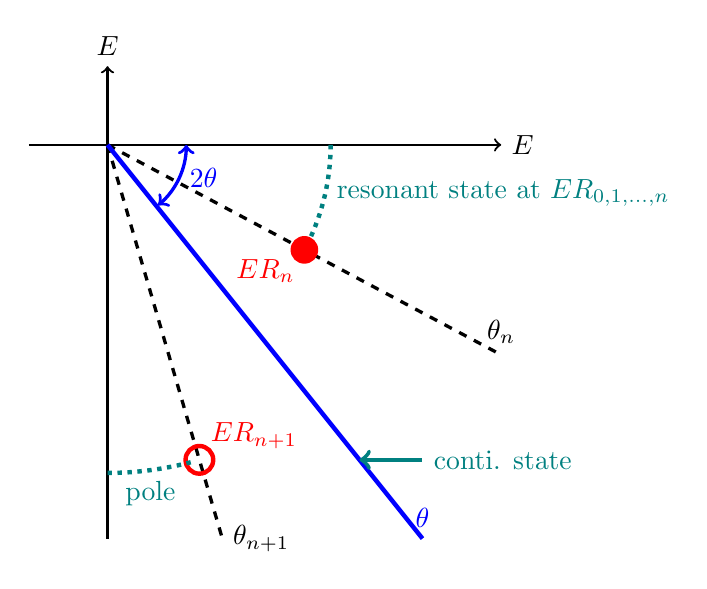
\begin{tikzpicture}
    \draw[->,thick] (-1,0) -- (5,0) node[right] {$\re E$};
    \draw[->,thick] (0,-5) -- (0,1) node[above] {$\im E$};
    %
    \draw[dashed,very thick] (0,0) -- (5,-8/3) node[above] {$\theta_n$};
    \draw[dashed,very thick] (0,0) -- (35/24,-5) node[right] {$\theta_{n+1}$};
    %
    \draw[ultra thick,blue] (0,0) -- (4,-5) node[above] {$\theta$};
    \draw[very thick,blue,<->] (1,0) arc(0:-50:1) node[midway,right] {$2\theta$};
    %
    \fill[red] (5/2,-4/3) circle(5pt) node[below left] {$\vsup{E}{R}_n$};
    \draw[red,ultra thick] (7/6,-4) circle(5pt) node[above right] {$\vsup{E}{R}_{n+1}$};
    %
    \draw[dotted,teal,ultra thick] (17/6,0) arc(0:-25:17/6) node[midway,right] {resonant state at $\vsup{E}{R}_{0,1,\dots,n}$};
    \draw[dotted,teal,ultra thick] (0,-25/6) arc(270:285:25/6) node[midway,below] {pole};
    \draw[<-,teal,ultra thick] (16/5,-4) -- (4,-4) node[right] {conti. state};
\end{tikzpicture}
    \caption{Schematic energy-plane picture of complex scaling. The complex-scaled continuum spectrum is rotated by $-2\theta$ (blue) from the positive real axis. We set $\theta_n<\theta<\theta_{n+1}$. Resonance poles at $\vsup{E_{n+1,n+2\dots}}{R}$ appear below the rotated cut, and Gamow states at $\vsup{E_{0,1,\dots,n}}{R}$ become regularized as discrete states.}
    \label{src:2512_24528:fig:theta_on_E}
\end{figure}
In what follows, we focus on the first resonance pole, $n=0$, and suppose that $\theta_0 < \theta < \theta_1$ to regularize the $n=0$ resonant wave function.
Note that the condition that $\theta_0<\theta<\theta_1$ provides an inequality depending on~$\lambda$, and so
\begin{align}
    - \frac{\im \vsup{E}{R}_0}{\re \vsup{E}{R}_0} < \tan 2\theta < - \frac{\im \vsup{E}{R}_1}{\re \vsup{E}{R}_1} .
\end{align}
One can find that
\begin{align}
    (\lambda < \lambda_0^- \,\lor\, \lambda_0^+ < \lambda)
    \quad \land \quad
    \lambda_1^- < \lambda < \lambda_1^+ ,
\end{align}
where, with $t=\tan^2(2\theta)$,
\begin{align}
    A_0&=\frac{1+t}{t},
    &A_1&=\frac{9+5t}{t},
    &B_1&=\frac{9+25t}{t},
    \\
    \lambda_0^\pm &= \frac{\beta^2 \hbar^2}{4m}
    \left[A_0\pm\sqrt{A_0^2-A_0}\right]
    \notag\\
    &\quad
    = \frac{\beta^2 \hbar^2}{4m}\frac{1 \pm \cos 2\theta}{\sin^2 2\theta} ,
    \\
    \lambda_1^\pm &= \frac{\beta^2 \hbar^2}{4m}
    \left[A_1\pm\sqrt{A_1^2-B_1}\right] .
\end{align}
Figure~\ref{src:2512_24528:fig:lambda_region} shows the functions~$\lambda_{0,1}^{\pm}$ with respect to~$\theta$ and indicates that $\lambda_0^+<\lambda<\lambda_1^+$ for small enough~$\theta$.
\begin{figure}[t]
    \centering
    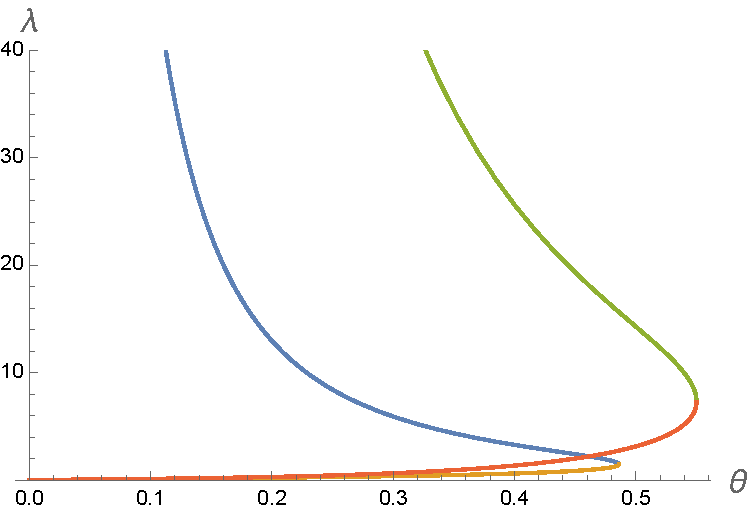
\includegraphics[width=0.5\columnwidth]{source_compendium/figures/2512_24528/lambda_region.pdf}
    \caption{$\lambda_{0,1}^\pm$ as functions of~$\theta$. $\frac{\beta^2\hbar^2}{4m}=1$. $\lambda$ should be above the blue curve which denotes $\lambda_0^+$ ($\lambda$ should be larger than it), or be below the orange curve which is $\lambda_0^-$ ($\lambda$ should be smaller than it). The green and red curves correspond to~$\lambda_1^+$ and~$\lambda_1^-$, respectively, and hence $\lambda$ should be inside the region between these curves. Eventually, we find that $\lambda$ is larger than~$\lambda_0^+$ and smaller than~$\lambda_1^+$ as long as $\theta$ is not too large.}
    \label{src:2512_24528:fig:lambda_region}
\end{figure}
\subsection{Classification of wave functions and self-orthogonality}
Let us change the parameter~$\lambda$ instead of~$\theta$ to follow the well-discussed approach to usual EPs in finite-dimensional non-Hermitian systems~\cite{Moiseyev2011NHQM}.
It is straightforward that changing $\lambda$ effectively deforms $\theta_n$ and so the wave function becomes ill defined outside $\lambda_0^{+}<\lambda<\lambda_1^{+}$ (see Fig.~\ref{src:2512_24528:fig:lambda_deformation}).
Then, the parameter $\lambda$ can contact with its EP, say $\vsub{\lambda}{bp}$, such that $\lim_{\lambda\to\vsub{\lambda}{bp}} \vsup{E}{R}_0 = \lim_{\lambda\to\vsub{\lambda}{bp}} \vsub{E}{CSM}(\theta) \equiv \vsub{E}{bp}$ for a value of~$E$.
\begin{figure}[t]
    \centering
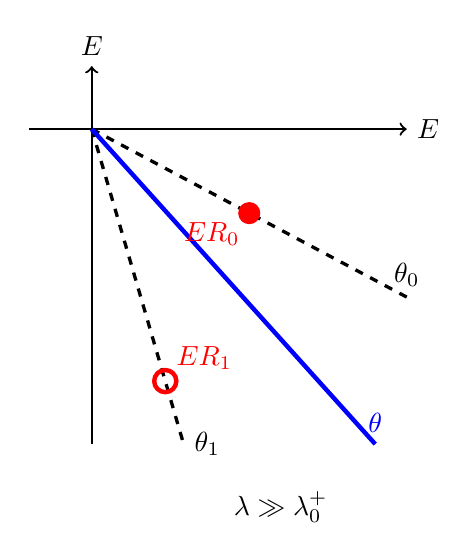
\begin{tikzpicture}[scale=0.8]
    \draw[->,thick] (-1,0) -- (5,0) node[right] {$\re E$};
    \draw[->,thick] (0,-5) -- (0,1) node[above] {$\im E$};
    %
    \draw[dashed,very thick] (0,0) -- (5,-8/3) node[above] {$\theta_0$};
    \draw[dashed,very thick] (0,0) -- (35/24,-5) node[right] {$\theta_{1}$};
    %
    \draw[ultra thick,blue] (0,0) -- (4.5,-5) node[above] {$\theta$};
    %
    \fill[red] (5/2,-4/3) circle(5pt) node[below left] {$\vsup{E}{R}_0$};
    \draw[red,ultra thick] (7/6,-4) circle(5pt) node[above right] {$\vsup{E}{R}_{1}$};
    %
    \node at (3,-6) {$\lambda\gg\lambda_0^{+}$};
\end{tikzpicture}
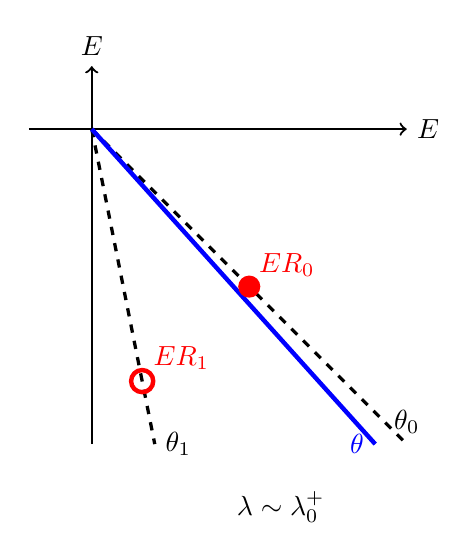
\begin{tikzpicture}[scale=0.8]
    \draw[->,thick] (-1,0) -- (5,0) node[right] {$\re E$};
    \draw[->,thick] (0,-5) -- (0,1) node[above] {$\im E$};
    %
    \draw[dashed,very thick] (0,0) -- (5,-5) node[above] {$\theta_0$};
    \draw[dashed,very thick] (0,0) -- (1,-5) node[right] {$\theta_{1}$};
    %
    \draw[ultra thick,blue] (0,0) -- (4.5,-5) node[left] {$\theta$};
    %
    \fill[red] (5/2,-5/2) circle(5pt) node[above right] {$\vsup{E}{R}_0$};
    \draw[red,ultra thick] (4/5,-4) circle(5pt) node[above right] {$\vsup{E}{R}_{1}$};
    %
    \node at (3,-6) {$\lambda\sim\lambda_0^{+}$};
\end{tikzpicture}
    \caption{Changing $\lambda$ and deformation of energy Riemann sheet. \textbf{Left:} For a moderate value of~$\lambda$, the resonant spectrum is completely isolated. \textbf{Right:} Near $\lambda_0^{+}$, the resonance pole is embedded into the continuum spectrum.}
    \label{src:2512_24528:fig:lambda_deformation}
\end{figure}
That is, precisely speaking, $\vsub{\lambda}{bp}$ is a root of the equation
\begin{align}
    \tan2\theta = - \frac{\im \vsub{E}{bp}}{\re \vsub{E}{bp}}
\end{align}
with the critical energy
\begin{align}
    \vsub{E}{bp} = \frac{\hbar^2\beta^2}{8m} \left[\sqrt{\frac{8m\vsub{\lambda}{bp}}{\beta^2 \hbar^2} - 1} - \rmi \right]^2.
\end{align}
We have
\begin{align}
    \vsub{\lambda}{bp} = \lambda_0^+ = \frac{\beta^2 \hbar^2}{4m}\frac{1 + \cos 2\theta}{\sin^2 2\theta}    
    = \frac{\beta^2 \hbar^2}{4m}\frac{1}{1-\cos2\theta} .
\end{align}
It is important to see the behavior of the wave function around $\vsub{\lambda}{bp}$.
Given $\lambda$, we have the Gamow state as $\vsub{\psi}{CSM}(\lambda)$.
If $\theta>\theta_0(\lambda)$ then $\vsub{\psi}{CSM}$ is one wave function associated with the resonance with~$\vsup{E}{R}_0$.
Thus, the resonance is just a pseudobound state in the regularized sense by CSM.
Here, going across~$\vsub{\lambda}{bp}$, one may take a drastic value of~$\lambda$ such that $\theta<\theta_0(\lambda)$.
It is trivial that $\vsub{\psi}{CSM}$ is divergent and there exists only a resonance pole at~$n=0$.
When $\theta=\theta_0(\lambda=\vsub{\lambda}{bp})$, any damping factor in~$\vsub{\psi}{CSM}$ disappears but the plane-wave behavior at the asymptotic region is left. Actually, this is identical to the scattering solution.
Figure~\ref{src:2512_24528:fig:lambda_contour} illustrates a contour of~$\lambda\in\mathbb{C}$ around~$\vsub{\lambda}{bp}$ and shows that $\vsub{\psi}{CSM}$ is convergent, divergent, or scattering.
The green region with the wavy lines implies the branch cut where the Gamow state should diverge; at the boundary (red line) a damping factor in the resonant wave function by CSM disappears.
\begin{figure}[t]
    \centering
\begin{tikzpicture}
    \fill[teal!10] (0,0) -- (6,-3) -- (10,-3) -- (10,0);
    \draw[teal,snake it] (5,-5/2) -- (8,0);
    \draw[teal,snake it] (3,-3/2) -- (5,0);
    \draw[teal,snake it] (1,-1/2) -- (2,0);
    %
    \draw[->] (-1,0) -- (10,0) node[right] {$\re E$};
    \draw[->] (0,-3) -- (0,1) node[above] {$\im E$};
    %
    \draw[red] (0,0) -- (6,-3);
    \fill (4,-2) circle(5pt) node[right] {$\vsub{E}{bp}$};
    %
    \draw[ultra thick,blue] (4,-2) circle(1);
    %
    \fill[blue] (4.5,-2.85) circle(3pt) node[below right] {$\lambda\mapsto\vsub{\psi}{CSM}$};
    %
    \node at (2,-3) {Convergent};
    \node[teal] at (7,-1) {Divergent};
    \node[red] at (9,-3) {Scattering (embedded)};
\end{tikzpicture}
    \caption{The resonance wave function as a function of~$\lambda$ around~$\vsub{\lambda}{bp}$. Given $\lambda$, we can see the behavior of~$\vsub{\psi}{CSM}(\lambda)$ with~$\vsup{E_0}{R}(\lambda)$. We consider the $\lambda$ contour around~$\vsub{\lambda}{bp}$ as depicted by the blue circle. Below the red line, $\vsub{\psi}{CSM}$ is convergent and a pseudobound state. Above it, the wave function is not regularized by CSM, so $\vsub{\psi}{CSM}$ diverges; this region is a kind of branch plane. At intersections between the red line and blue curve, the resonance is embedded into the continuum spectrum, and its wave function is identical to the scattering solution.}
    \label{src:2512_24528:fig:lambda_contour}
\end{figure}
To follow explicitly how a resonance pole approaches and coalesces with the complex-scaled continuum, we use a momentum-bin discretization of the continuum spectrum. The method and the associated notation are summarized in Sec.~\ref{src:2512_24528:sec:bin_method}, so that the present section can focus directly on the resulting branch-point structure and its physical consequences.
The resonant wave function $\vsupb{\psi}{R}{CSM}(\lambda)$ with $\lambda\neq\vsub{\lambda}{bp}$ is an independent solution of the non-Hermitian linear differential equation.
We also have the momentum-binned states $\vsupb{\psi}{bin}{CSM}(n,\lambda)$ as the independent scattering solutions~$\vsupb{\psi}{conti}{CSM}$ in a bin.
Originally, the linear eigenvalue problem possesses
\begin{align}
    \int \vsupb{\psi}{R}{CSM}(\lambda) \vsupb{\psi}{R}{CSM}(\lambda) \rmd x &= 1 , \\
    \int \vsupb{\psi}{bin}{CSM}(n',\lambda) \vsupb{\psi}{bin}{CSM}(n,\lambda) \rmd x &= \delta_{n'n}, \\
    \int \vsupb{\psi}{R}{CSM}(\lambda) \vsupb{\psi}{bin}{CSM}(n,\lambda) \rmd x &= 0 .
\end{align}
Note that the binned states are normalized with a Kronecker delta, which makes the relevant formulas technically simpler and the branch structure easier to track explicitly. By contrast, the original continuum states are normalized with a Dirac delta, and this distribution normalization tends to obscure the algebraic steps and their physical interpretation in the present context.
Let us consider the limit as~$\lambda\to\vsub{\lambda}{bp}$.
From the exact solution, we can find that
\begin{align}
    &\lim_{\lambda\to\vsub{\lambda}{bp}} \vsup{E_0}{R}(\lambda)
    = \vsub{E}{bp} ,\\
    &\lim_{\lambda\to\vsub{\lambda}{bp}} \vsupb{\psi}{R}{CSM}(\lambda)
    = \vsupb{\psi}{conti}{CSM}(\vsub{k}{bp},\vsub{\lambda}{bp}).
    \label{src:2512_24528:eq:lim_res_is_conti}
\end{align}
Thus, there exists only one general scattering solution with the identical eigenenergy.
Now, exchanging the limit and the inner product (integral over~$x$) is contradictory.
This is because
\begin{align}
    &\int \lim_{\lambda\to\vsub{\lambda}{bp}}\vsupb{\psi}{R}{CSM}(\lambda) \vsupb{\psi}{bin}{CSM}(n,\lambda) \rmd x
    = \int \vsupb{\psi}{conti}{CSM}(\vsub{k}{bp},\lambda) \vsupb{\psi}{bin}{CSM}(n,\lambda) \rmd x \neq 0
    &&
    \text{$\exists n$} ,\\
    &\lim_{\lambda\to\vsub{\lambda}{bp}}\int \vsupb{\psi}{R}{CSM}(\lambda) \vsupb{\psi}{bin}{CSM}(n,\lambda) \rmd x
    = \lim_{\lambda\to\vsub{\lambda}{bp}} 0 = 0
    &&
    \text{$\forall n$} .
\end{align}
Therefore, the biorthogonality cannot be ensured.
To remedy this, it is natural in non-Hermitian quantum systems to introduce \textit{left} eigenvectors in addition to the \textit{right} (usual) eigenvectors.
Without exchanging the limit and integral, all right continuum states~$\vsupb{\psi}{bin}{CSM}$ are orthogonal to a left scattering solution associated with the resonance, $\lim_{\lambda\to\vsub{\lambda}{bp}}\vsupb{\psi}{R}{CSM}\sim\vsupb{\psi}{bin}{CSM}(\vsub{n}{bp})$ with $\exists \vsub{n}{bp}$.\footnote{For simplicity, one may rewrite it as~$(\vsub{\psi}{Left}(\vsub{n}{bp}),\vsub{\psi}{Right}(\vsub{n}{bp}))=0$ for the degenerate solution~$\psi(\vsub{n}{bp})$ if no confusion arises.}
This is called the self-orthogonality (no biorthogonal basis).
This is a special phenomenon in non-Hermitian linear algebra so that not only the eigenvalues but also the eigenvectors are degenerate.
The Hamiltonian is nondiagonalizable but has a Jordan block.
\subsection{Geometric phase near resonance pole}
Here the geometric phase is defined for adiabatic transport along a closed loop in parameter space. At the exceptional point itself the eigenvectors coalesce and the Berry connection is not well defined; our results therefore pertain to loops that encircle the EP (the associated branch point), capturing the monodromy or holonomy.
Moiseyev's ansatz of non-Hermitian energy near EP \cite{Moiseyev2011NHQM} is given by
\begin{align}
    \vsub{E}{CSM}^\theta(\lambda) = \vsub{E}{bp} + \alpha \sqrt{\lambda - \vsub{\lambda}{bp}} + O(\lambda),
    \label{src:2512_24528:eq:moiseyev}
\end{align}
and we define $\lambda$ as
\begin{align}
    \lambda = \vsub{\lambda}{bp} + R \rme^{\rmi \phi} 
    \quad(R\ll1).
\end{align}
The parameter $\alpha$ in Moiseyev's ansatz is introduced to label the branch (Riemann sheet) of the analytically continued resonance energy. It is fixed once the continuation path and the continuity condition of the resonance pole are specified, and it is not a tunable parameter. The final holonomy or Berry phase is insensitive to $\alpha$ beyond this discrete sheet identification.
Note that the square root of~$\lambda$ around~$\vsub{\lambda}{bp}$ comes from its branch order~$2$, that is, if $p$ wave functions coalesce into an EP then $(\lambda-\vsub{\lambda}{bp})^{1/p}$.\footnote{It looks hard to count the number of continuum states. Nevertheless, since there is one corresponding resonant pole/state, the rank of the projection operator to the resonance is definitely equal to one. This is the same situation as the spectrum intensity in Breit--Wigner peak of the Feshbach resonance. Thus, the associated continuum spectrum is unidentified, but one continuum state can be responsible for the EP phenomenon; it provides $p=2$.} $\alpha$ is a complex parameter.
Let us consider the geometric phase of the wave function in the CSM based on Moiseyev's ansatz. We rewrite the solution of Eq.~\eqref{src:2512_24528:eq:CSM-eq} as 
\begin{align}
    &\vsub{\psi}{CSM}(k,\lambda,x')= (1-\xi^2)^{-\frac{\rmi k}{2\beta}} 
    F\left( -\frac{\rmi k}{\beta}-s, -\frac{\rmi k}{\beta}+s+1, -\frac{\rmi k}{\beta}+1, \frac{1-\xi}{2} \right),
    \label{src:2512_24528:eq:CSM-sol}
\end{align}
where $k=-\rmi \beta\kappa=\sqrt{2m\vsub{E^\theta}{csm}(\lambda)}/\hbar$ and the $k$ and $\lambda$ dependencies are written explicitly on the right-hand side. For simplicity, we discuss the geometric phase by using the asymptotic forms of the solution represented as (for instance, see Ref.~\cite{MorikawaOgawa2025PTEP})
\begin{align}
    &\vsub{\psi}{CSM}(k,\lambda,x')\xrightarrow{x\to\infty}4^{-\frac{\rmi k}{2\beta}} \rme^{\rmi kx'} ,
    \\  
    &\vsub{\psi}{CSM}(k,\lambda,x')\xrightarrow{x\to-\infty}
    4^{-\frac{\rmi k}{2\beta}}
    \left[\rme^{-\rmi kx'}\mathcal A_-(k)+\rme^{\rmi kx'}\mathcal A_+(k)\right].
    \label{src:2512_24528:eq:CSM-asy}
\end{align}
Here the two connection coefficients are
\begin{align}
    \mathcal A_-(k)
    &=\frac{\Gamma(1-\frac{\rmi k}{\beta})\Gamma(\frac{\rmi k}{\beta})}
    {\Gamma(1+s)\Gamma(-s)},
    \\
    \mathcal A_+(k)
    &=\frac{\Gamma(1-\frac{\rmi k}{\beta})\Gamma(-\frac{\rmi k}{\beta})}
    {\Gamma(-\frac{\rmi k}{\beta}-s)
     \Gamma(-\frac{\rmi k}{\beta}+s+1)}.
\end{align}
The above solution corresponds to a continuum state.
To avoid some mathematical difficulties, we discretize the continuum state by using the momentum-bin method. We assume that Moiseyev's ansatz applies to a wavenumber as well if $|\lambda-\vsub{\lambda}{bp}|\ll1$, and we define the discretized wavenumber $k_n$ by 
\begin{align}
    k_n &= \vsub{k}{bp}+\alpha'_n\sqrt{\lambda-\vsub{\lambda}{bp}}
    \label{src:2512_24528:eq:dis-kn1}
    \\
    &= \vsub{k}{bp}+\alpha'_nR^{\frac{1}{2}}\rme^{\frac{\rmi \phi}{2}} ,
    \label{src:2512_24528:eq:dis-kn2}
\end{align}
where $\vsub{k}{bp}=\sqrt{2m\vsub{E}{bp}}/\hbar$. Using $k_n$, we see the geometric phase as follows.
\subparagraph{\textbf{Case I:} $x\to\infty$}
    The momentum-binned state at $x\to\infty$ is given by
    \begin{align}
        \vsupb{\psi}{bin}{CSM}(n,\lambda,x') &\to \frac{1}{\sqrt{\Delta k}} \int_{k_n}^{k_{n+1}} 4^{-\frac{\rmi k}{2\beta}} \rme^{\rmi kx'}\rmd k
        \notag\\
        &= \frac{1}{\sqrt{\Delta k}} \frac{\rme^{\left(-\frac{\rmi \ln{4}}{2\beta}+\rmi x'\right)k_{n+1}}-\rme^{\left(-\frac{\rmi \ln{4}}{2\beta}+\rmi x'\right)k_{n}}}{-\frac{\rmi \ln{4}}{2\beta}+\rmi x'} .
    \end{align} 
    Substituting Eq.~\eqref{src:2512_24528:eq:dis-kn1} into the above equation, we obtain a compact expression by defining
    $\zeta=-\rmi \ln4/(2\beta)+\rmi x'$:
    \begin{align}
        \vsupb{\psi}{bin}{CSM}(n,\lambda,x')
        &\to\frac{\rme^{\zeta \vsub{k}{bp}}}
        {\sqrt{\Delta k}\,\zeta}
        \left\{
        \rme^{\zeta\alpha'_{n+1}\sqrt{\lambda-\vsub{\lambda}{bp}}}
        -\rme^{\zeta\alpha'_{n}\sqrt{\lambda-\vsub{\lambda}{bp}}}
        \right\}.
        \label{src:2512_24528:eq:psi_inf_asymp_lambda}
    \end{align}
    Provided that the exponents of the terms in the brace brackets on the right-hand side are sufficiently small, the Taylor expansion of the asymptotic wave function is given as
    \begin{align}
        \vsupb{\psi}{bin}{CSM}(n,\lambda,x') &\approx\frac{1}{\sqrt{\Delta k}}
        \frac{\rme^{\zeta \vsub{k}{bp}}}{\zeta}\,\zeta
        (\alpha'_{n+1}-\alpha'_n)\sqrt{\lambda-\vsub{\lambda}{bp}} \notag\\
        &= \frac{1}{\sqrt{\Delta k}}
        \rme^{\zeta \vsub{k}{bp}}
        (\alpha'_{n+1}-\alpha'_n)\sqrt{\lambda-\vsub{\lambda}{bp}}.
    \end{align}
    Here noting that $\Delta k=(\alpha'_{n+1}-\alpha'_n)\sqrt{\lambda-\vsub{\lambda}{bp}}$ and substituting Eq.~\eqref{src:2512_24528:eq:dis-kn2},
    \begin{align}
        \vsupb{\psi}{bin}{CSM}(n,\lambda,x') &\approx \rme^{\zeta \vsub{k}{bp}}\sqrt{\alpha'_{n+1}-\alpha'_n}R^{\frac{1}{4}}\rme^{\rmi \frac{\phi}{4}} .
        \label{src:2512_24528:eq:psi_inf_asymp}
    \end{align}
    The factor $\rme^{\rmi \frac{\phi}{4}}$ indicates that $\vsupb{\psi}{bin}{CSM}(n,\lambda(\phi=0),x')|_{x\to\infty}=\vsupb{\psi}{bin}{CSM}(n,\lambda(\phi=8\pi),x')|_{x\to\infty}$.
\subparagraph{\textbf{Case II:} $x\xrightarrow{}-\infty$}
    Now, $\vsub{E^\theta}{CSM}(\lambda)$ is very close to $\vsub{E}{bp}$, i.e., the resonant energy. Thus, by the Siegert boundary condition \cite{Siegert:1939}, the coefficient of the second term in Eq.~\eqref{src:2512_24528:eq:CSM-asy} is negligible, and that term can be omitted. That is, the condition 
    \begin{align}
        \frac{\Gamma(1-\frac{\rmi k}{\beta})\Gamma(-\frac{\rmi k}{\beta})}{\Gamma(-\frac{\rmi k}{\beta}-s)\Gamma(-\frac{\rmi k}{\beta}+s+1)}\approx0 
    \end{align}
    implies $\frac{\rmi k}{\beta}\approx s+1$.\footnote{Note that the complex energy of the resonance at the fourth quadrant can be given by the condition $\frac{\rmi k}{\beta}=s+1$, while the complex energy of the anti-resonance at the first quadrant comes from $\frac{\rmi k}{\beta}=-s$.}
    Consequently, the asymptotic form reduces to 
    \begin{align}
        \vsub{\psi}{CSM}(k,\lambda,x')\xrightarrow{x\to-\infty} 4^{-\frac{\rmi k}{2\beta}} \rme^{-\rmi kx'} ,
    \end{align}
    and its discrete form is 
    \begin{align}
        \vsupb{\psi}{bin}{CSM}(n,\lambda,x') &\xrightarrow{x\to-\infty}
        \frac{1}{\sqrt{\Delta k}}\int_{k_n}^{k_{n+1}} 4^{-\frac{\rmi k}{2\beta}} \rme^{-\rmi kx'} \rmd k
        \notag\\
        &\ \qquad = \frac{1}{\sqrt{\Delta k}} \frac{\rme^{\left(-\frac{\rmi \ln{4}}{2\beta}-\rmi x'\right)k_{n+1}}-\rme^{\left(-\frac{\rmi \ln{4}}{2\beta}-\rmi x'\right)k_{n}}}{-\frac{\rmi \ln{4}}{2\beta}-\rmi x'} .
    \end{align}
    This is essentially the same as \textbf{Case I}, and a similar calculation yields the factor $\rme^{\rmi \frac{\phi}{4}}$.\footnote{Alternatively, if the coefficient of the first term in Eq.~\eqref{src:2512_24528:eq:CSM-asy} is retained exactly, Euler’s reflection formula leads to the asymptotic form
    \begin{align}
        4^{-\frac{\rmi k}{2\beta}} \rme^{-\rmi kx'} \frac{\rmi \sin(\pi s)}{\sinh(\frac{\pi k}{\beta})} .
    \end{align}
    Using the formula
    \begin{align}
        \frac{1}{\sinh(\frac{\pi k}{\beta})} = 2 \sum_{n=0}^{\infty} \rme^{-(2n+1)\frac{\pi k}{\beta}} \qquad \left(\re \frac{\pi k}{\beta} >0\right) ,
    \end{align}
    the momentum-binned state is modified as
    \begin{align}
        \vsupb{\psi}{bin}{CSM}(n,\lambda,x') &\xrightarrow{x\to-\infty} 2\frac{\sin(\pi s)}{\sqrt{\Delta k}} \sum_{n=0}^{\infty} \int_{k_n}^{k_{n+1}} \rme^{\left(-\frac{\rmi \ln{4}}{2\beta}-\rmi x'-\frac{(2n+1)\pi}{\beta}\right)k}\rmd k
        \notag\\
        &\ \qquad = 2\frac{\sin(\pi s)}{\sqrt{\Delta k}} \sum_{n=0}^{\infty} \frac{\rme^{\left(-\frac{\rmi \ln{4}}{2\beta}-\rmi x'-\frac{(2n+1)\pi}{\beta}\right)k_{n+1}}-\rme^{\left(-\frac{\rmi \ln{4}}{2\beta}-\rmi x'-\frac{(2n+1)\pi}{\beta}\right)k_{n}}}{-\frac{\rmi \ln{4}}{2\beta}-\rmi x'-\frac{(2n+1)\pi}{\beta}} .
    \end{align}
    Thus, the same calculation as in \textbf{Case I} gives $\rme^{\rmi \frac{\phi}{4}}$ as an overall factor.}
    Thus, the same periodicity condition, $\vsupb{\psi}{bin}{CSM}(n,\lambda(\phi=0),x')|_{x\to-\infty}=\vsupb{\psi}{bin}{CSM}(n,\lambda(\phi=8\pi),x')|_{x\to-\infty}$, is satisfied.
Incorporating \textbf{Case I} and \textbf{Case II}, when we consider the contour depicted in Fig.~\ref{src:2512_24528:fig:lambda_contour}, that is, encircling the critical energy~$\vsub{E}{bp}$ by changing~$\lambda$ (or $\phi$), the wave function should have the $8\pi$ periodicity (branch order is $4$). This periodicity or branch structure is quite universal in non-Hermitian quantum mechanics with a $2\times 2$ Jordan block. It is, however, much more nontrivial and remarkable that the additional branch structure arises due to the discretized momentum-bin size~$\Delta k$, and so it essentially depends on the continuous (unbounded) parameter~$k$ after removing the cutoff scale.
Here the additional branch structure is traced to the square-root normalization factor~$1/\sqrt{\Delta k}$
in Eq.~\eqref{src:2512_24528:eq:psi_inf_asymp_lambda} that arises from momentum-bin discretization. While this introduces an apparent dependence on the bookkeeping parameter $\alpha_n$
[cf. Eq.~\eqref{src:2512_24528:eq:psi_inf_asymp}], the associated branch choice does not affect the final result: it is precisely this square-root branch that guarantees that the discretized formulation reproduces the Berry phase.
To gain more physical insight, let us see what has happened by the $\phi$ rotation.
Figure~\ref{src:2512_24528:fig:psi_on_lambda} shows how to encircle $\vsub{E}{bp}$ by the current rotation.
The region A denotes the area where $\vsupb{\psi}{R}{CSM}(\lambda(\phi))$ is normalizable, while the region B implies that any resonance is not regularized by CSM.
At the boundary between A and B, the resonant state becomes the continuum one as Eq.~\eqref{src:2512_24528:eq:lim_res_is_conti}.
Also we set $\arg\alpha$ as the below panel in Fig.~\ref{src:2512_24528:fig:psi_on_lambda} so that Moiseyev's ansatz~\eqref{src:2512_24528:eq:moiseyev} becomes $E(\lambda^{-})$ when $\phi=0$.
In effect, now, we can decompose the complex-energy regions as
\begin{align}
    E_{\pm} = \vsub{E}{bp} \pm \alpha R^{\frac{1}{2}} \rme^{\frac{\rmi \phi}{2}} 
    \qquad
    \phi\in[0,2\pi].
\end{align}
Here, the resonant state possesses its complex eigenenergy by~$E_+$ in this convention.
Suppose that $\vsupb{\psi}{R}{CSM}(\lambda(0|_A))$ and $\vsupb{\psi}{conti}{CSM}(\lambda(0|_B))$ are taken as the exact solution~\eqref{src:2512_24528:eq:CSM-sol} (i.e., \textit{their overall phase conform to that of the explicit expression}).
\begin{figure}[t]
    \centering
\begin{tikzpicture}[scale=0.9]
    \fill[teal!10] (0,0) -- (6,-3) -- (8,-3) -- (8,0);
    \draw[teal,snake it] (5,-5/2) -- (8,0);
    \draw[teal,snake it] (3,-3/2) -- (5,0);
    \draw[teal,snake it] (1,-1/2) -- (2,0);
    %
    \draw[->] (0,0) -- (8,0) node[right] {$\re E$};
    \draw[->] (0,-3) -- (0,1) node[above] {$\im E$};
    %
    \draw[red] (0,0) -- (6,-3);
    \fill (4,-2) circle(5pt) node[right] {$\vsub{E}{bp}$};
    %
    \draw[ultra thick,blue] (4,-2) circle(1);
    %
    \fill[blue] (4.9,-2.45) circle(3pt) node[left] {$\lambda^{+}$};
    \fill[blue] (3.1,-1.55) circle(3pt) node[right] {$\lambda^{-}$};
    \draw[ultra thick,red,dotted,->] (5,-2.8) -- (5.5,-2);
    \draw[ultra thick,red,dotted,->] (3,-1) -- (2.5,-1.8);
    %
    \node at (2,-3) {A: $\vsupb{\psi}{R}{CSM}$};
    \node[teal] at (8,-1) {B: $\vsupb{\psi}{conti}{CSM}$};
    \node[red] at (6,-3.5) {$\lim_{\lambda\nearrow}\vsupb{\psi}{R}{CSM}=\vsupb{\psi}{conti}{CSM}$};
\end{tikzpicture}\\
\begin{tikzpicture}[scale=0.9]
    \draw[very thick] (0,0) circle(0.1) node[right] {$\vsub{E}{bp}$};
    \fill[blue] (-2,0) circle(0.1) node[below left] {$\lambda^{-}$};
    \fill[blue] (2,0) circle(0.1) node[below right] {$\lambda^{+}$};
    %
    \draw[ultra thick,teal,->] (2,0) arc(0:180:2);
    \node[left,teal] at (0,2.2) {$\phi\in[0,2\pi]$};
    \node[teal] at (0,0.5) {$E_-=\vsub{E}{bp}-\alpha R^{\frac{1}{2}}\rme^{\frac{\rmi \phi}{2}}$};
    %
    \draw[ultra thick,->] (-2,0) arc(180:360:2);
    \node[right] at (0,-2.2) {$\phi\in[0,2\pi]$};
    \node at (0,-0.6) {$E_+=\vsub{E}{bp}+\alpha R^{\frac{1}{2}}\rme^{\frac{\rmi \phi}{2}}$};
    %
    \draw[ultra thick,red,dashed,->] (-0.2,0) -- (-1.95,0) node[left] {$\arg\alpha$};
\end{tikzpicture}
    \caption{The resonance and continuum wave functions in the complex energy plane. The contour around~$\vsub{E}{bp}$ is depicted by the blue circle. Below the red line, i.e., in the region A, $\vsupb{\psi}{R}{CSM}$ is well defined. Otherwise, in the region B, we focus on~$\vsupb{\psi}{conti}{CSM}$. At intersections between the red line and blue curve, say $\lambda^{+}$ and~$\lambda^{-}$, the resonance is identical to the continuum state~$\vsupb{\psi}{conti}{CSM}$ along the limit of~$\lambda$ as the left and/or right eigenfunction. We set the argument of~$\alpha$ as the below panel so that Moiseyev's ansatz~\eqref{src:2512_24528:eq:moiseyev} becomes $E(\lambda^{-})$ when $\phi=0$.}
    \label{src:2512_24528:fig:psi_on_lambda}
\end{figure}
First, we start from an intersection point in the region A defined by~$\phi=0$, so $\vsupb{\psi}{R}{CSM}(\lambda(0|_A))=\vsupb{\psi}{R}{CSM}(\lambda^{-})$.
Second, we deform $\lambda$ near the vicinity of another intersection, that is, $\lambda(2\pi|_A)=\lambda^{+}$. Note that the overall factor~$\rme^{\frac{\rmi \phi}{4}}$ exists in each wave function, by which the dilated resonant wave function differs from the continuum state. We thus use the continuity condition as
\begin{align}
    \vsupb{\psi}{R}{CSM}(\lambda(2\pi|_A))=\rme^{\frac{\rmi \pi}{2}}\vsupb{\psi}{conti}{CSM}(\lambda(0|_B))=\rmi \vsupb{\psi}{conti}{CSM}(\lambda(0|_B)) .
\end{align}
Next, by deformation in the region B, we have
\begin{align}
    \vsupb{\psi}{conti}{CSM}(\lambda(2\pi|_B))=\rme^{\frac{\rmi \pi}{2}}\vsupb{\psi}{R}{CSM}(\lambda(0|_A))=\rmi \vsupb{\psi}{R}{CSM}(\lambda(0|_A)) .
\end{align}
If the complex energy rotates once, the wave function acquires a minus sign:
\begin{align}
    \vsupb{\psi}{R}{CSM}(\lambda(4\pi|_A))
    = - \vsupb{\psi}{R}{CSM}(\lambda(0|_A)) .
\end{align}
This is the reason why $\phi$ has the $4\times2\pi$ periodicity.
We have observed the nontrivial Berry phase induced by the resonance pole as an EP.
\subsection{Chern characteristic and monodromy renormalization}
Finally, we consider a simple extension: the Chern-type characteristic of the quantum resonance pole as an EP in the parameter space.
We show that it is associated with a resonance branch point in the $\lambda$-parameter space, and a renormalization viewpoint on the monodromy (holonomy) when continuum normalization becomes distributional.
\subsubsection{Biorthogonal connection and bin-regularized holonomy}
We first define an Abelian connection for a (generically) non-Hermitian eigenproblem.
It is natural to define the Chern connection by
\begin{align}
    \mathcal{A}^\theta(\lambda)
    \equiv \rmi  \int \vsupb{\psi}{bi(Left)}{CSM} \frac{\partial}{\partial\lambda} \vsupb{\psi}{(Right)}{CSM} \rmd x
    = \rmi  ( \psi(\lambda), \partial_\lambda \psi(\lambda)).
\end{align}
Here, $\vsup{\psi}{(Left)}$ denotes a left eigenvector, and $\vsup{\psi}{(Right)}$ is an associated right eigenvector (biorthogonal partner); those are corresponding to~$\vsupb{\psi}{R}{CSM}$ or~$\vsupb{\psi}{conti,bin}{CSM}$ in an appropriate way.
We then define the holonomy around the branch point $\vsub{\lambda}{bp}$ as
\begin{align}
    \gamma &\equiv \vsub{\oint}{bp} \mathcal{A}^\theta(\lambda) \rmd \lambda,
    &
    c_1 &\equiv \frac{1}{2\pi}\gamma,
    \label{src:2512_24528:eq:holonomy_chern_character}
\end{align}
where $c_1$ is a Chern-type characteristic (first Chern number when the underlying line bundle is globally well defined).
We next evaluate $\gamma$ within the momentum-bin regularization and focus on the most singular contribution in $\lambda-\vsub{\lambda}{bp}$.
For simplicity, suppose that from the asymptotic relation in Eq.~\eqref{src:2512_24528:eq:psi_inf_asymp}
\begin{align}
    \frac{\partial}{\partial\lambda}\vsupb{\psi}{bin}{CSM}(n,\lambda,x')
    \approx \frac{1}{4}\frac{1}{\lambda-\vsub{\lambda}{bp}}\vsupb{\psi}{bin}{CSM}(n,\lambda,x') .
\end{align}
In this bin-level estimate, the left or right distinction affects only nonsingular gauge choices and does not modify the holonomy; hence we suppress it for notational simplicity.\footnote{More precisely, the holonomy $\gamma$ is invariant under $\psi\to \rme^{\rmi \chi(\lambda)}\psi$ and the corresponding transformation of $\vsup{\psi}{bi}$, so the leading singular piece is sufficient for $\gamma$.}
Then, a nontrivial Abelian phase of holonomy around the resonance pole is obtained if $n=\vsub{n}{bp}$ by
\begin{align}
    \gamma(\vsub{n}{bp}) &\equiv \vsub{\oint}{bp} \mathcal{A}^\theta(\vsub{n}{bp},\lambda) \rmd \lambda \\
    &= \rmi  \vsub{\oint}{bp} \int \vsupb{\psi}{bin(Left)}{CSM}(\vsub{n}{bp},\lambda,x') \frac{\partial}{\partial\lambda} \vsupb{\psi}{bin(Right)}{CSM}(\vsub{n}{bp},\lambda,x') \rmd x \rmd \lambda \notag\\
    &= \rmi  \vsub{\oint}{bp} \frac{1}{4}\frac{1}{\lambda-\vsub{\lambda}{bp}} \rmd \lambda
    = \frac{\pi}{2} .
\end{align}
The four-rotations invariance is reflected in $\rme^{\rmi \gamma}\in\mathbb{Z}_4$. The Chern characteristic suffers from the fractionality of its naive Chern number; the corresponding characteristic $c_1=\gamma/2\pi=1/4$ is fractional in this bin-regularized sense.
That is, it indicates that the resonance eigenstate under CSM does not define a globally rigid (single-valued) line bundle over the punctured
$\lambda$-plane without passing to a branched cover.
\subsubsection{Continuum limit: Two sources of ill definedness}
So far, the momentum-bin method and the exact solution of the inverted Rosen--Morse potential have enabled us to provide the explicit estimates in all of our observations.
Averaging continuum states within a momentum bin is a technique in finite volume regularization.
The continuum eigenvectors are, however, defined intrinsically by a distribution-valued construction (rigged Hilbert space, \vN\ ring with affiliated operators, semi-infinite measure, and so on).
Even in the formal continuum spectrum, the physical picture remains intact and is not particularly sensitive to the choice of geometric path, so we do not confine the discussion to geometric paths alone.
On the other hand, the definition of~$\mathcal{A}(\lambda)$ becomes quite subtle due to the plausible normalization factor as~$\delta(0)$ for the continuum states.
Hence, in this section, the vector-bundle structure induced by~$\lambda$ is not straightforwardly applied to the continuum case.
Here is a short summary:
The problem is divided into (A) inner products of the continuum states and (B) the number of those.
(A) Continuum eigenvectors are $\delta$-function normalized, and inner products produce regulator-dependent singular factors such as $\delta(0)$ (or its derivatives). This affects the very meaning of $\mathcal{A}^\theta(\lambda)$ unless a specific regularization (finite volume box, wave-packet, test-function, etc.) is fixed.
(B) Even after choosing a regulator, the set of continuum states is uncountable and the associated bundlelike structure over parameter space is not automatically inherited straightforwardly.
To make the appearance of (A) explicit, in general, we have an asymptotic form of the scattering/resonant solution near the resonance pole
\begin{align}
    \vsupb{\psi}{as}{CSM}(k,\lambda,x') =
    \begin{cases}
        \frac{1}{\sqrt{2\pi}} \rme^{\rmi kx'} & \re x'\gg0, \\
        \frac{1}{\sqrt{2\pi}} \rme^{-\rmi kx'} & \re x'\ll0,
    \end{cases}
\end{align}
where $k=\vsub{k}{bp}+\alpha'\sqrt{\lambda-\vsub{\lambda}{bp}}$ and this is $\delta$-function normalized.
With attention to the self-orthogonality, we obtain
\begin{align}
    \mathcal{A}^\theta(\lambda)
    &= \rmi  \lim_{k'\to k,\lambda'\to\lambda}
    \int \vsupb{\psi}{as(Left)}{CSM}(k',\lambda',x') \frac{\partial}{\partial\lambda} \vsupb{\psi}{as(Right)}{CSM}(k,\lambda,x') \rmd x \\
    &= \rmi  \lim_{k'\to k,\lambda'\to\lambda}
    \frac{\partial k}{\partial\lambda} \frac{\partial}{\partial k}
    \int \vsupb{\psi}{as(Left)}{CSM}(k',\lambda',x')  \vsupb{\psi}{as(Right)}{CSM}(k,\lambda,x') \rmd x\\
    &= \rmi \left(\frac{\alpha'}{2\sqrt{\lambda-\vsub{\lambda}{bp}}} + \frac{\partial\alpha'}{\partial\lambda} \sqrt{\lambda-\vsub{\lambda}{bp}}\right) \delta'(0),
    \label{src:2512_24528:eq:berry_as_delta}
\end{align}
where we have assumed that $\alpha'=\alpha'(\lambda)$ to be $\lambda$ dependent.
Here $\delta'(0)$ is a shorthand for the regulator-dependent singular factor arising from differentiating the continuum overlap; its precise meaning depends on the chosen regularization scheme (e.g., box normalization or wave-packet regularization).
The naive connection requires renormalization/regularization data in the
continuum.
\subsubsection{Monodromy renormalization: Fixing the physical holonomy}
$\gamma$ takes measurements of the monodromy around the EP.
Now, we implement the monodromy renormalization method in Ref.~\cite{Morikawa:2025ezl} as a way to separate physical content
from regulator dependence.
Let us remove the microscopic circle around~$\vsub{\lambda}{bp}$ with the radius~$R$.
Then, the physical holonomy being kept $\pi/2$, i.e., $\vsup{\gamma}{phys}=\pi/2$, the \textit{bare} holonomy depends on~$R$ as
\begin{align}
    \vsup{\gamma}{phys} = \frac{\vsup{\gamma}{bare}(R)}{Z_{\gamma}(R)} .
\end{align}
$Z_\gamma(R)$ plays the role of a renormalization factor that absorbs regulator dependence [including distributional normalization factors such as $\delta(0)$ or $\delta'(0)$].
Still, $\vsup{\gamma}{bare}$ can be divergent by~$\delta(0)$, but only the renormalized monodromy is observable.
Notice that it appears that $\alpha$ ($\alpha'$) is a measure of the number of continuum states along the $E$ ($k$) contour.
In fact, the structure of $k=\vsub{k}{bp}+\alpha' R^{\frac{1}{2}}\rme^{\frac{\rmi \phi}{2}}$ suggests that the coefficient $\alpha'$ controls how many continuum states effectively contribute along the $k$ contour (equivalently, along the energy contour).
Motivated by this, we introduce a redefinition (running) of $\alpha'(\lambda)$ such that the singular factor $\delta'(0)$ is
absorbed into $\alpha'$.
We impose the renormalization-group-type condition
\begin{align}
    \alpha' + 2\frac{\partial\alpha'}{\partial\lambda}(\lambda-\vsub{\lambda}{bp}) = \frac{\alpha_0}{2\sqrt{\lambda-\vsub{\lambda}{bp}}\delta'(0)} \label{src:2512_24528:eq:renor_group}
\end{align}
for finite~$\alpha_0$, and the solution is given by
\begin{align}
    \alpha'(\lambda) = \frac{\alpha_0}{4\delta'(0)} \frac{\ln(\lambda-\vsub{\lambda}{bp})}{\sqrt{\lambda-\vsub{\lambda}{bp}}} + \frac{\text{(const.)}}{\sqrt{\lambda-\vsub{\lambda}{bp}}} .
\end{align}
Under this redefinition, the $\delta$ function from the connection can be absorbed by the \textit{renormalization} of~$\alpha'$.\footnote{$\delta'(0)$ should not be interpreted as a literal number: the connection is meaningful only after specifying a regularization and/or
considering smeared states (test functions), and in the present discussion its dependence is absorbed into renormalized quantities.
For instance, in a box of length $L$ one has $\delta(0)\sim L/2\pi$ (and derivatives thereof depend on boundary
conditions), while in a wave-packet regularization $\delta$ is replaced by a narrow function of width $\epsilon$.
The renormalization group equation should therefore be read as a compact way to track this regulator dependence.}
Then, the resulting holonomy becomes finite and proportional to $\alpha_0$:
\begin{align}
    \vsup{\gamma}{bare}(R)=\frac{\pi}{2}\alpha_0.
\end{align}
The physical monodromy is kept fixed while the regulator dependence is absorbed into $Z_{\gamma}(R)=\alpha_0$ and the running parameter $\alpha'(\lambda)$.
Eventually, while~$\vsup{\gamma}{phys}=\pi/2$ in this way, the bin-level result and the continuum viewpoint can be unified within a renormalization framework, providing a consistent physical picture of monodromy around a resonance branch point in the presence of continuum normalization singularities.
%\section{Stokes phenomenon under complex-scaling method}
\subsection{Complex-scaled continuum states in momentum-bin method}\label{src:2512_24528:sec:bin_method}
Since treating the continuum spectrum entails substantial technical difficulties, we introduce a discretization scheme; in particular, applying it also to the CSM makes subsequent computations considerably more tractable.
In this calculation module, we briefly review the momentum-bin method and fix our notation, mainly to make the paper self-contained.
\subsubsection{Hermitian quantum mechanics}
It is complicated to treat continuum states because they are intrinsically $\delta$-function normalized. Let $\phi(k,x)$ denote a continuum state with a momentum $k$, whose orthogonality is determined by
\begin{align}
    \int \phi^*(k',x) \phi(k,x) \rmd x = \delta(k'-k) .
\end{align}
We therefore discretize the continuum states using the momentum-bin method, in which the resulting bin states provide an accurate representation of the continuum states in realistic nuclear reaction calculations~\cite{Yahiro2012CDCC}. In this method, a continuum state is averaged over the width of the momentum bin $\Delta k$.
It is then natural to define a discretized state by
\begin{align}
    \Hat{\phi}_n (x) = \frac{1}{\sqrt{\Delta k}} \int_{k_n}^{k_{n+1}}\phi(k,x) \rmd k,
    \qquad
    k_{n+1} - k_n = \Delta k,\,
    n\in\mathbb{Z}.
\end{align}
The orthogonality of the discretized states is shown as
%\footnote{One may use the bracket notation as~$\dualpair{\Hat\phi_{n'}}{\Hat\phi_n}=\delta_{n'n}$.}
\begin{align}
    \int\Hat{\phi}_{n'}^*(x) \Hat{\phi}_n (x) \rmd x &= \frac{1}{\Delta k} \int_{k'_{n'}}^{k'_{n'+1}} \int_{k_n}^{k_{n+1}} \delta(k'-k) \rmd k' \rmd k
    \notag\\
    &= \delta_{n'n} .
\end{align}
One may use the bracket notation as
\begin{equation}
    \dualpair{\Hat\phi_{n'}}{\Hat\phi_n}=\delta_{n'n}.
\end{equation}
Moreover, a Hamiltonian $h$ is diagonalized with regard to~$\Hat{\phi}_n (x)$ as follow:
in scattering problem, from the Schr\"odinger equation
\begin{align}
    h \phi(k,x) = \frac{\hbar^2k^2}{2m} \phi(k,x) ,
\end{align}
we find that
\begin{align}
    \int\Hat{\phi}_{n'}^*(x) h \Hat{\phi}_n (x) \rmd x &= \frac{1}{\Delta k} \int_{k'_{n'}}^{k'_{n'+1}} \int_{k_n}^{k_{n+1}} \frac{\hbar^2 k^2}{2m} \delta(k'-k) \rmd k' \rmd k
    \notag\\
    &= \Hat{\epsilon}_n \delta_{n'n} ,
\end{align}
where
\begin{align}
    \Hat{\epsilon}_n \equiv \frac{1}{\Delta k} \int_{k_n}^{k_{n+1}} \frac{\hbar^2 k^2}{2m}\rmd k .
\end{align}
The relation between $\Hat{\phi}_n(x)$ and $\phi(k,x)$ is now represented as
\begin{align}
    \int \phi^*(k,x) \Hat{\phi}_n(x) \rmd x &= 
    \begin{cases}
        \frac{1}{\sqrt{\Delta k}} & k_n \le k \le k_{n+1} ,\\
        \ \ \ 0 & \text{otherwise} .
    \end{cases}
\end{align}
As a simple example, the momentum-bin discretization of a plane wave
\begin{align}
    \frac{1}{\sqrt{\Delta k}} \int_{k_n}^{k_{n+1}} \rme^{\rmi kx} \rmd k = \frac{1}{\sqrt{\Delta k}} \frac{\rme^{\rmi k_{n}x}-\rme^{\rmi k_{n+1}x}}{\rmi x}
\end{align}
falls off as $1/x$ for large $x$.
\subsubsection{Complex-scaled Hamiltonian}
The momentum-bin method is well-established in Hermitian quantum mechanics. In this section, we extend it to non-Hermitian quantum mechanics. Let us consider the complex-scaled continuum state $\phi^{\theta}(k,x)$, which is a solution of the complex-scaled Hamiltonian $h^{\theta}$.
It is natural to consider that the discretization of the state is given by
\begin{align}
    \Hat{\phi}_n^{\theta} (x) &= \frac{1}{\sqrt{\Delta k}} \int_{k_n}^{k_{n+1}} \phi^{\theta}(k,x) \rmd k .
\end{align}
The biorthogonal state of $\phi^{\theta}(k,x)$ is $\phi^{*\theta}(k,x)$ (see Chap.\ 6.1 in Ref.~\cite{Moiseyev2011NHQM}). Thus, the biorthogonal state of $\Hat{\phi}_n^{\theta} (x)$ is represented as
\begin{align}
    \vsup{\Hat{\phi}_n}{bi,\theta} (x) &\equiv \frac{1}{\sqrt{\Delta k}} \int_{k_n}^{k_{n+1}} \phi^{*\theta}(k,x) \rmd k .
\end{align}
Then, the orthogonality of the scaled and discretized state is shown as
%\footnote{The corresponding bracket notation is given as~$(\Hat\phi_{n'},\Hat\phi_n)=\delta_{n'n}$, which is the bilinear inner product.}
\begin{align}
    \int \vsup{\Hat{\phi}_{n'}}{bi,\theta} (x) \Hat{\phi}_n^{\theta} (x) \rmd x &= \frac{1}{\Delta k} \int_{k'_{n'}}^{k'_{n'+1}} \int_{k_n}^{k_{n+1}} \left\{ \int \phi^{*\theta}(k',x) \phi^{\theta}(k,x) \rmd x \right\} \rmd k'\rmd k
    \notag\\
    &=\frac{1}{\Delta k} \int_{k'_{n'}}^{k'_{n'+1}} \int_{k_n}^{k_{n+1}} \delta(k'-k) \rmd k'\rmd k
    \notag\\
    &=\delta_{n'n}.
\end{align}
The corresponding bracket notation is given as
\begin{equation}
    (\Hat\phi_{n'},\Hat\phi_n)=\delta_{n'n}, 
\end{equation}
which is the bilinear inner product.

\subsection*{Laboratory checkpoint}
Before moving to the next stage, perform the following checks without copying
the displayed final answer.
\begin{enumerate}
  \item Expand the resonance condition to second order at the EP and derive the square-root branches and the associated Jordan vector.
  \item Verify self-orthogonality with the complex-symmetric bilinear product and relate it to the derivative of the pole condition.
  \item Repeat the encircling calculation at two momentum-bin widths and separate the bin-dependent norm from the limiting holonomy.
\end{enumerate}
